\documentclass[10pt,aspectratio=169]{beamer}

% ---------- Theme ----------
\usetheme{Madrid}
\usepackage[T1]{fontenc}
\usepackage[utf8]{inputenc}
\usepackage{amsmath,amssymb}
\usepackage{booktabs}
\usepackage{makecell}
\usepackage{graphicx}
\usepackage{xcolor}
\usepackage{tikz}
\usepackage{pgfplots}
\pgfplotsset{compat=1.18}

% Colors
\definecolor{accent}{HTML}{2563EB}
\definecolor{accent2}{HTML}{DC2626}
\definecolor{accent3}{HTML}{059669}
\definecolor{good}{HTML}{059669}
\definecolor{bad}{HTML}{DC2626}

\setbeamercolor{frametitle}{bg=accent,fg=white}
\setbeamercolor{title separator}{fg=accent}
\setbeamercolor{progress bar}{fg=accent}

% Compact spacing
\setbeamertemplate{itemize item}{\textcolor{accent}{$\bullet$}}
\setbeamertemplate{itemize subitem}{\textcolor{accent}{$\circ$}}
\setbeamertemplate{navigation symbols}{}

% ---------- Title ----------
\title{Part E: Mortgage Survival Analysis}
\subtitle{Competing Risks\enspace$\cdot$\enspace Time-Varying Cox\enspace$\cdot$\enspace Neural Models\enspace$\cdot$\enspace Scenario Analysis}
\author{Yueqi Lin}
\institute{MTH 9877 --- Interest Rate and Credit Models\\Baruch College, Spring 2026}
\date{May 13, 2026}

% =========================================================================
\begin{document}

% ---- Global title --------------------------------------------------------
\begin{frame}[plain]
    \titlepage
\end{frame}

% =========================================================================
\section{E(i): Competing Risks}
% =========================================================================

\begin{frame}
    \vfill
    \begin{center}
        {\color{accent}\rule{0.28\linewidth}{1.2pt}}\\[0.7em]
        {\Large\bfseries Part E(i)}\\[0.5em]
        {\large Competing Risks: Prepayment vs.\ Default}\\[0.4em]
        {\small Kaplan--Meier vs.\ Aalen--Johansen\enspace$\cdot$\enspace
                Cause-Specific Cox\enspace$\cdot$\enspace Fine--Gray}\\[0.7em]
        {\color{accent}\rule{0.28\linewidth}{1.2pt}}
    \end{center}
    \vfill
\end{frame}

\begin{frame}{Prepaid and default are competing risks.}
    \begin{center}
        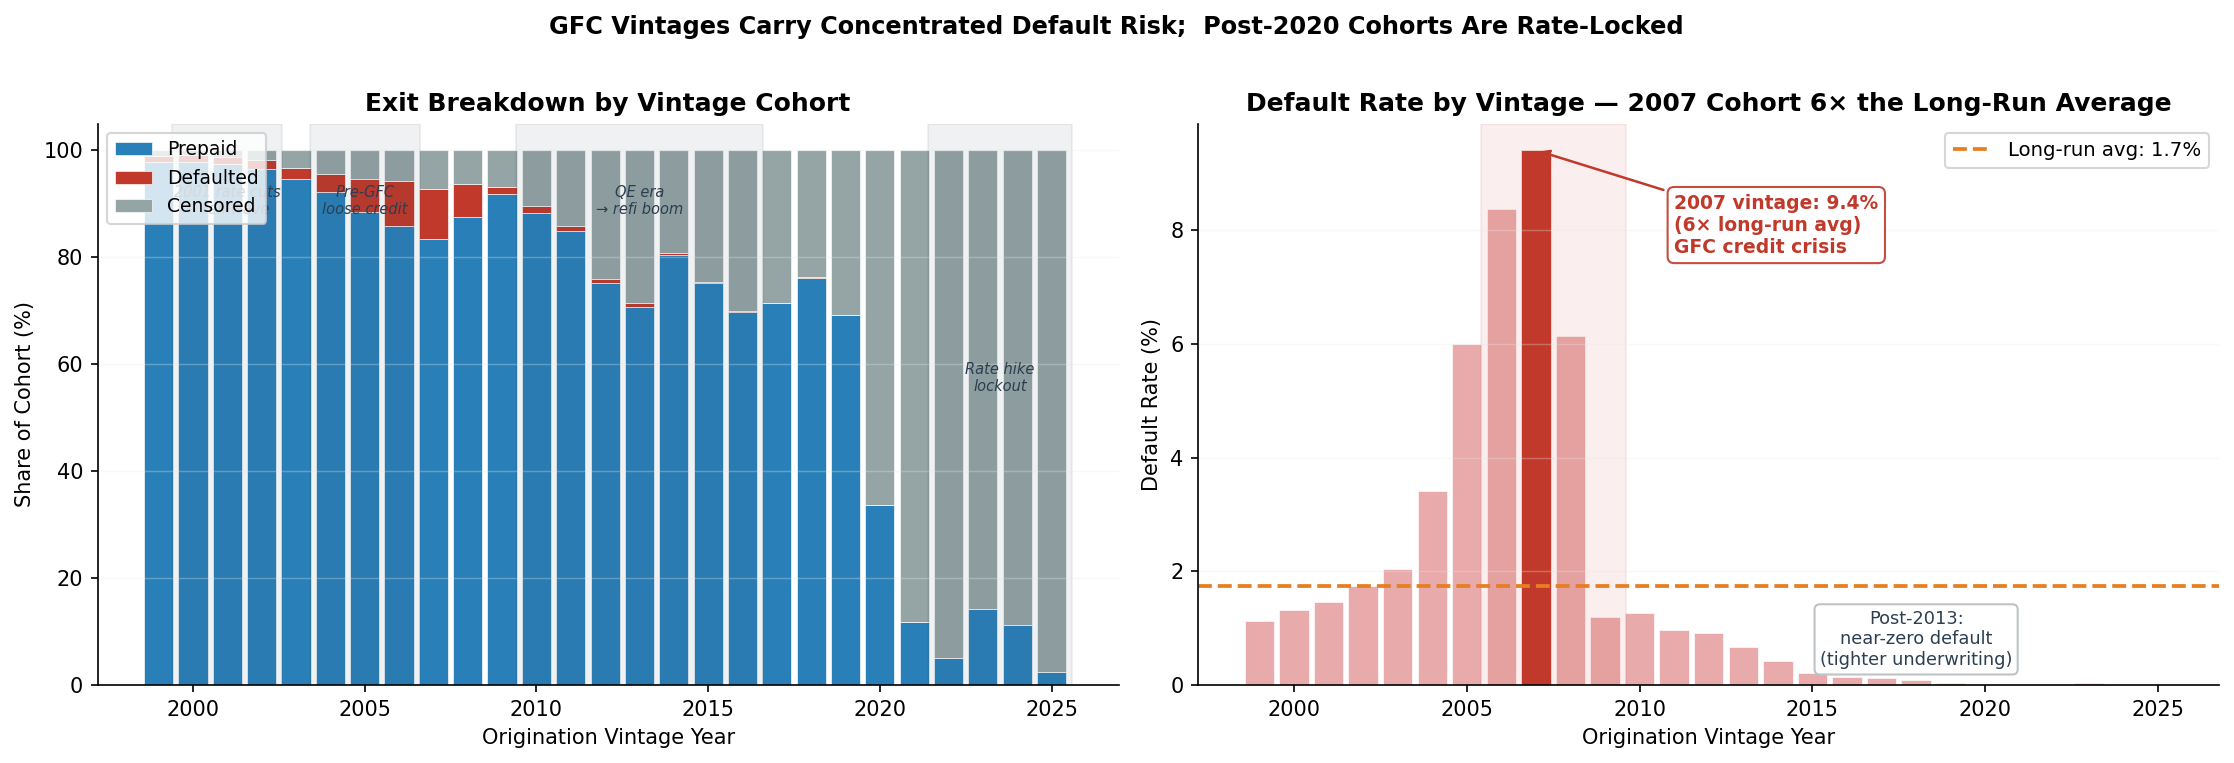
\includegraphics[height=0.40\textheight,keepaspectratio]{processed/E1_eda_vintage}\\[0.15em]
        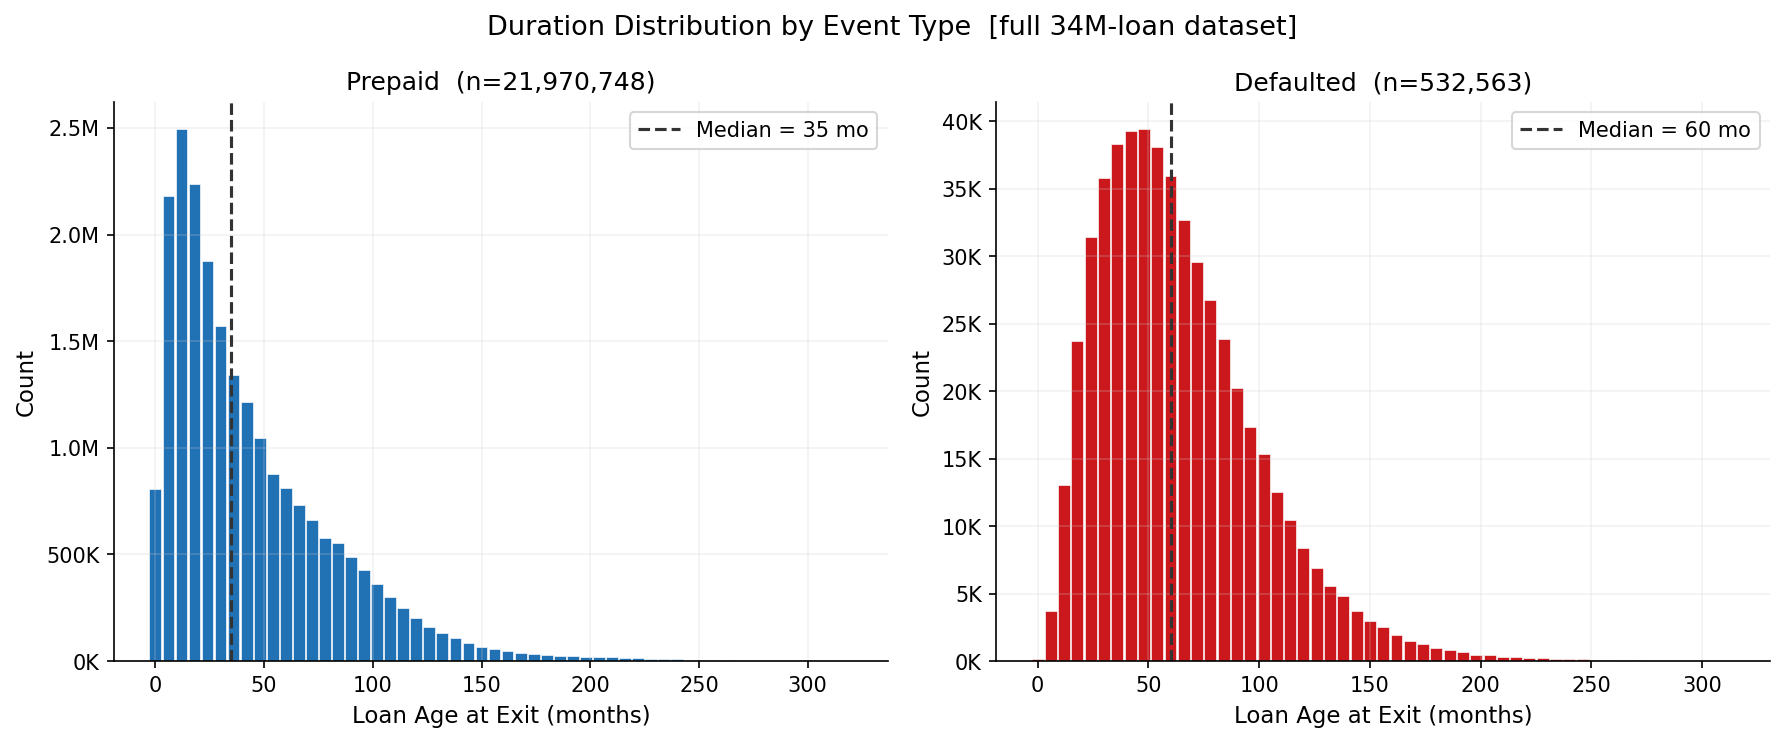
\includegraphics[height=0.40\textheight,keepaspectratio]{processed/E1_eda_duration}
    \end{center}
\end{frame}

\begin{frame}{Kaplan--Meier vs.\ Aalen--Johansen.}
    \begin{columns}[T,onlytextwidth]
        \column{0.48\textwidth}
        \begin{block}{Kaplan--Meier}
        \[
            \hat{F}^{(k)}_{\mathrm{KM}}(t)
            = 1 - \prod_{t_j \le t}\!\left(1 - \frac{d_{j}^{(k)}}{n_j^{\mathrm{KM}}}\right)
        \]
        \vspace{0.1em}
        \small
        \begin{tabular}{@{}ll@{}}
            $d_j^{(k)}$ & cause-$k$ exits at $t_j$ \\[2pt]
            $n_j^{\mathrm{KM}}$ & \textbf{risk set excluding competing-event loans}\\[2pt]
        \end{tabular}
        \end{block}

        \column{0.48\textwidth}
        \begin{block}{Aalen--Johansen}
        \[
            \hat{F}_k(t) = \sum_{t_j \le t} \hat{S}(t_j^{-})\cdot \frac{d_{kj}}{n_j}
        \]
        \vspace{0.1em}
        \small
        \begin{tabular}{@{}ll@{}}
            $d_{kj}$        & cause-$k$ exits at $t_j$ \\[2pt]
            $n_j$           & risk set including all exits \\[2pt]
            $\hat{S}(t_j^-)$ & \textbf{overall survival just before $t_j$} \\[2pt]
        \end{tabular}
        \end{block}
    \end{columns}
    \vspace{0.6em}
    \begin{center}
        \small
        KM: competing exits censored $\Rightarrow$ denominator too small $\Rightarrow$ each increment inflated.\\[3pt]
        AJ: $\hat{S}(t_j^-)$ shrinks with every exit $\Rightarrow$ $\hat{F}^{(\mathrm{pre})} + \hat{F}^{(\mathrm{def})} + \hat{S} = 1$ always.
    \end{center}
\end{frame}

\begin{frame}{Aalen--Johansen CIF: coherent probability partition.}
    \begin{columns}[c,onlytextwidth]
        \column{0.64\textwidth}
        \begin{center}
            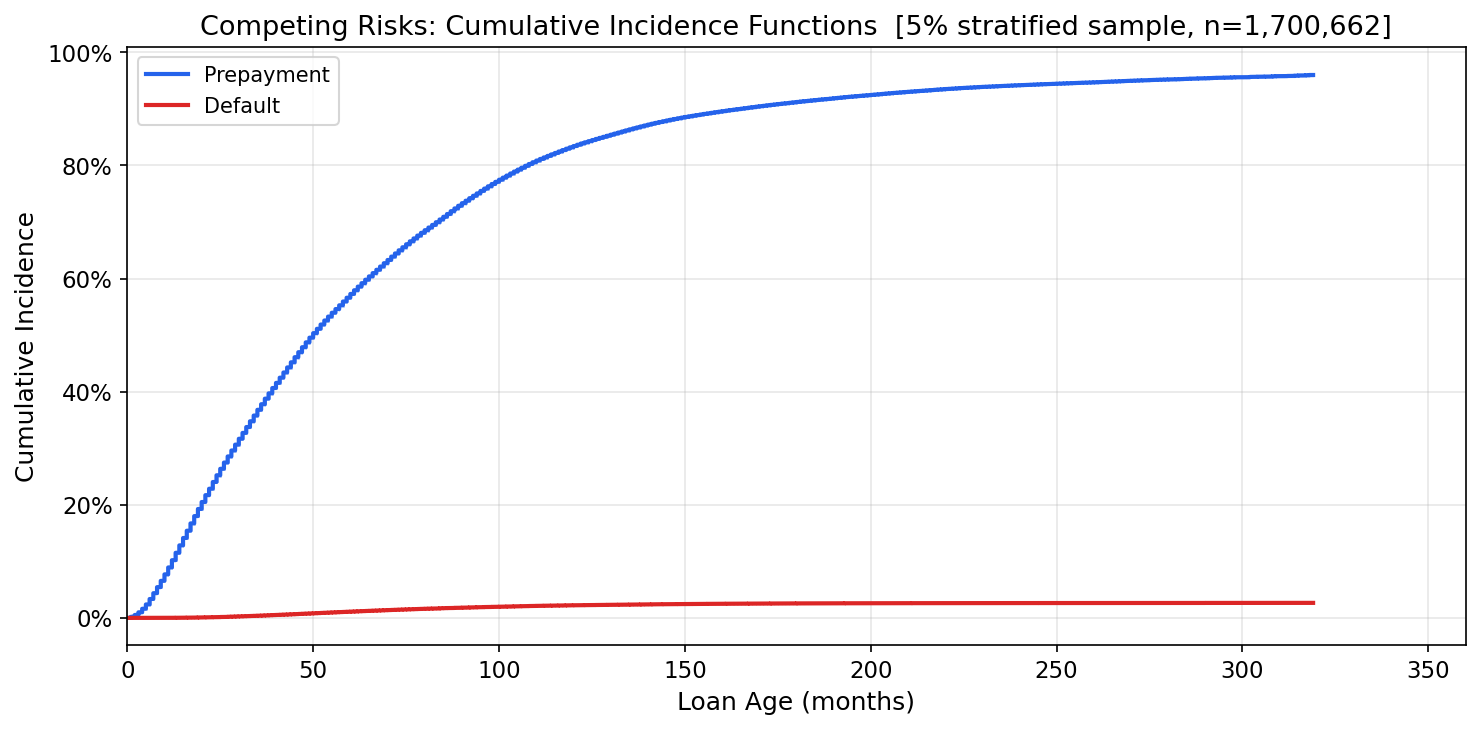
\includegraphics[width=\linewidth]{processed/E1_competing_risks_cif}
        \end{center}

        \column{0.34\textwidth}
        \begin{center}
        \vspace{1em}
        \small
        \textbf{Cumulative Incidence Function}\\[3pt]
        $F_k(t) = P(\text{exit by }t,\ \text{cause }k)$\\[10pt]
        \textbf{Aalen--Johansen CIF partition}\\[4pt]
        \begin{tabular}{lccc}
            \toprule
            & Prepaid & Default & Active \\
            \midrule
            5 yr  & 61.4\% & 1.1\% & 37.6\% \\
            10 yr & 83.3\% & 2.2\% & 14.5\% \\
            20 yr & 91.8\% & 3.1\% &  5.1\% \\
            \bottomrule
        \end{tabular}
        \end{center}
    \end{columns}
\end{frame}

\begin{frame}{KM overstates prepayment by up to 2.2\,pp.}
    \begin{center}
        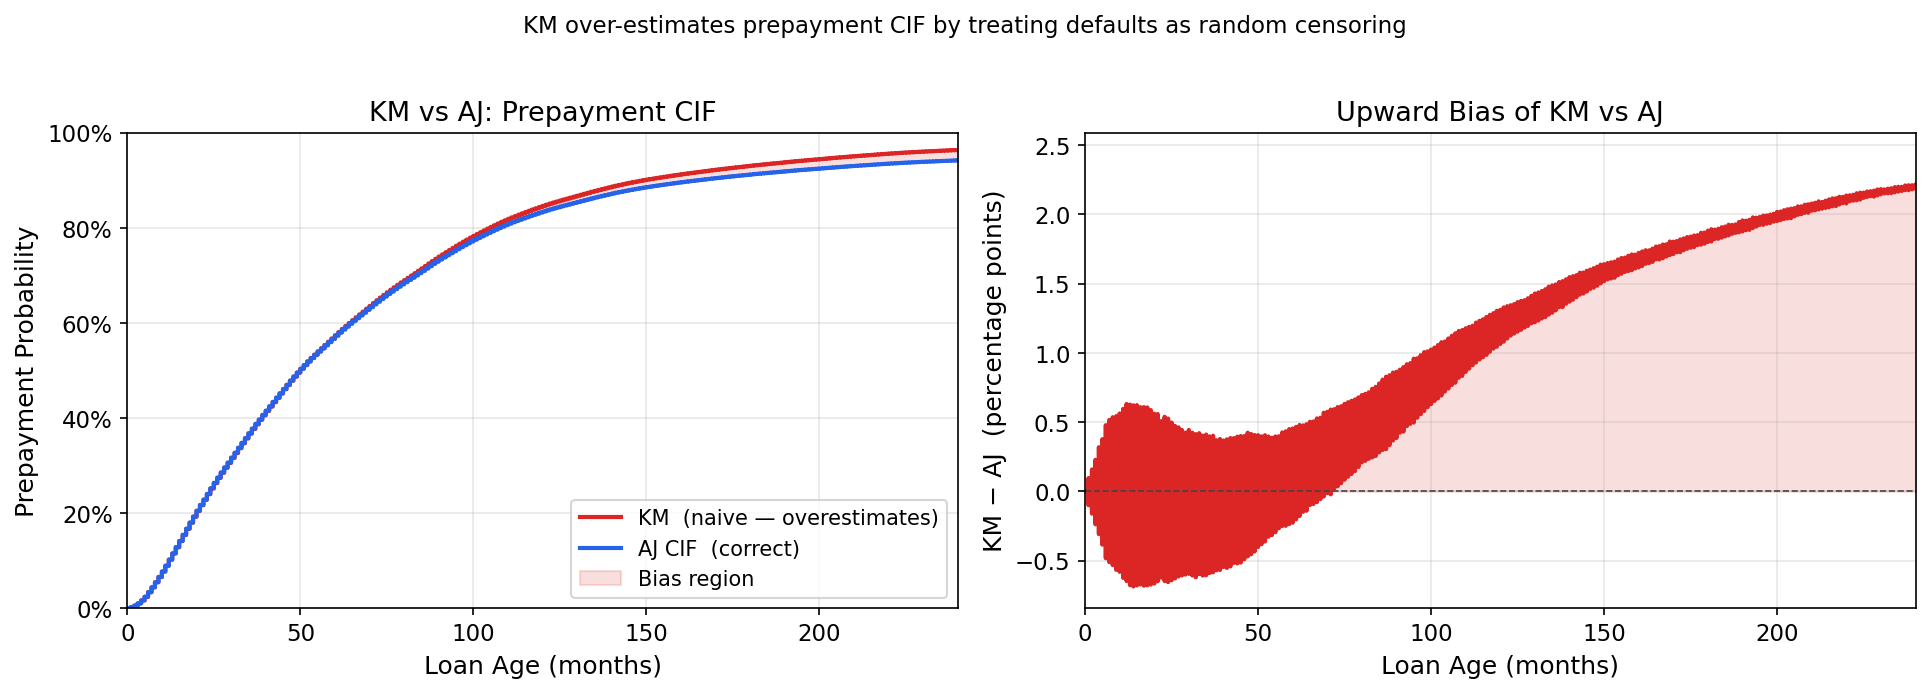
\includegraphics[width=0.82\linewidth]{processed/E1_km_vs_aj_bias}
    \end{center}
    \vspace{-0.3em}
    \begin{center}
        \small
        \textbf{KM overstatement of prepayment probability}\\[4pt]
        \begin{tabular}{lccc}
            \toprule
            Horizon & $\hat{F}_{\mathrm{KM}}$ & $\hat{F}_{\mathrm{AJ}}$ & Bias \\
            \midrule
            5 yr  & 61.9\% & 61.4\% & $+$0.45 pp \\
            10 yr & 84.6\% & 83.3\% & $+$1.31 pp \\
            20 yr & 93.4\% & 91.8\% & $+$2.23 pp \\
            \bottomrule
        \end{tabular}
    \end{center}
\end{frame}

\begin{frame}{FICO and LTV separate default, not prepayment.}
    \begin{center}
        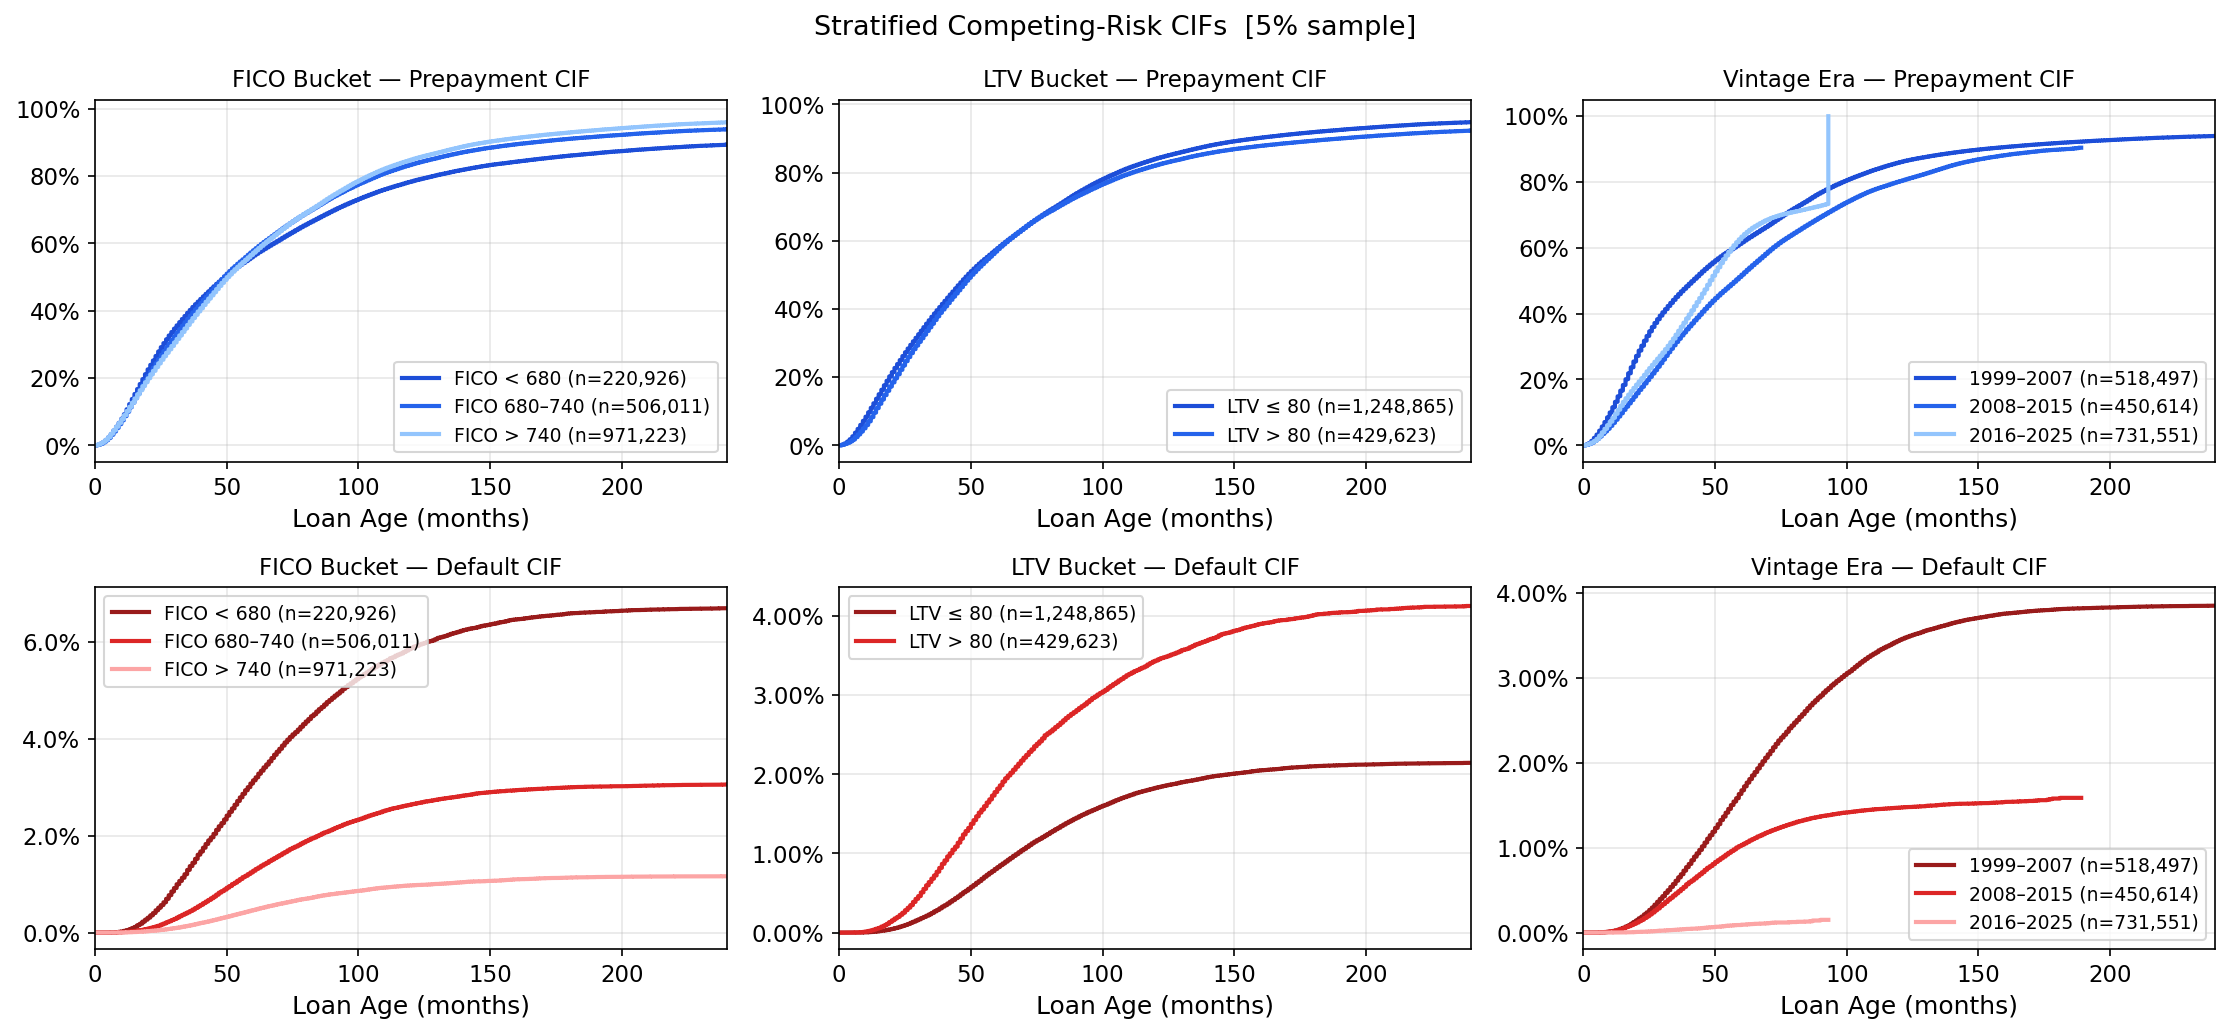
\includegraphics[height=0.78\textheight,keepaspectratio]{processed/E1_stratified_cif}
    \end{center}
\end{frame}

\begin{frame}{Cause-specific Cox model.}
    \begin{columns}[T,onlytextwidth]
        \column{0.54\textwidth}
        \begin{block}{Cause-Specific Cox}
        \[
            h_k(t \mid \mathbf{x}) = h_{0k}(t)\,\exp\!\bigl(\boldsymbol{\beta}_k^\top\mathbf{x}\bigr),
            \quad k \in \{\mathrm{pre},\,\mathrm{def}\}
        \]
        \[
            \ell(\boldsymbol{\beta}_k) = \sum_{i:\,E_i=k}
            \!\Biggl[
                \boldsymbol{\beta}_k^\top \mathbf{x}_i
                - \log\!\sum_{j\in\mathcal{R}(t_i)}
                e^{\boldsymbol{\beta}_k^\top\mathbf{x}_j}
            \Biggr]
        \]
        \end{block}
        \vspace{0.4em}
        \small
        $\mathcal{R}(t_i)$: all loans still active just before $t_i$.\\[3pt]
        Competing-cause exits are \textbf{censored} --- they leave
        $\mathcal{R}(t)$ without contributing to $\ell$.

        \column{0.42\textwidth}
        \small\vspace{0.4em}

        \normalsize\textbf{Additional features}\\[6pt]
        \small
        \textbf{Max Delinquency} --- months past due over loan life\\[6pt]
        \textbf{Ever 90+ DQ} --- binary flag for severe delinquency
    \end{columns}
\end{frame}

\begin{frame}{Opposite covariate effects by cause.}
    \begin{center}
        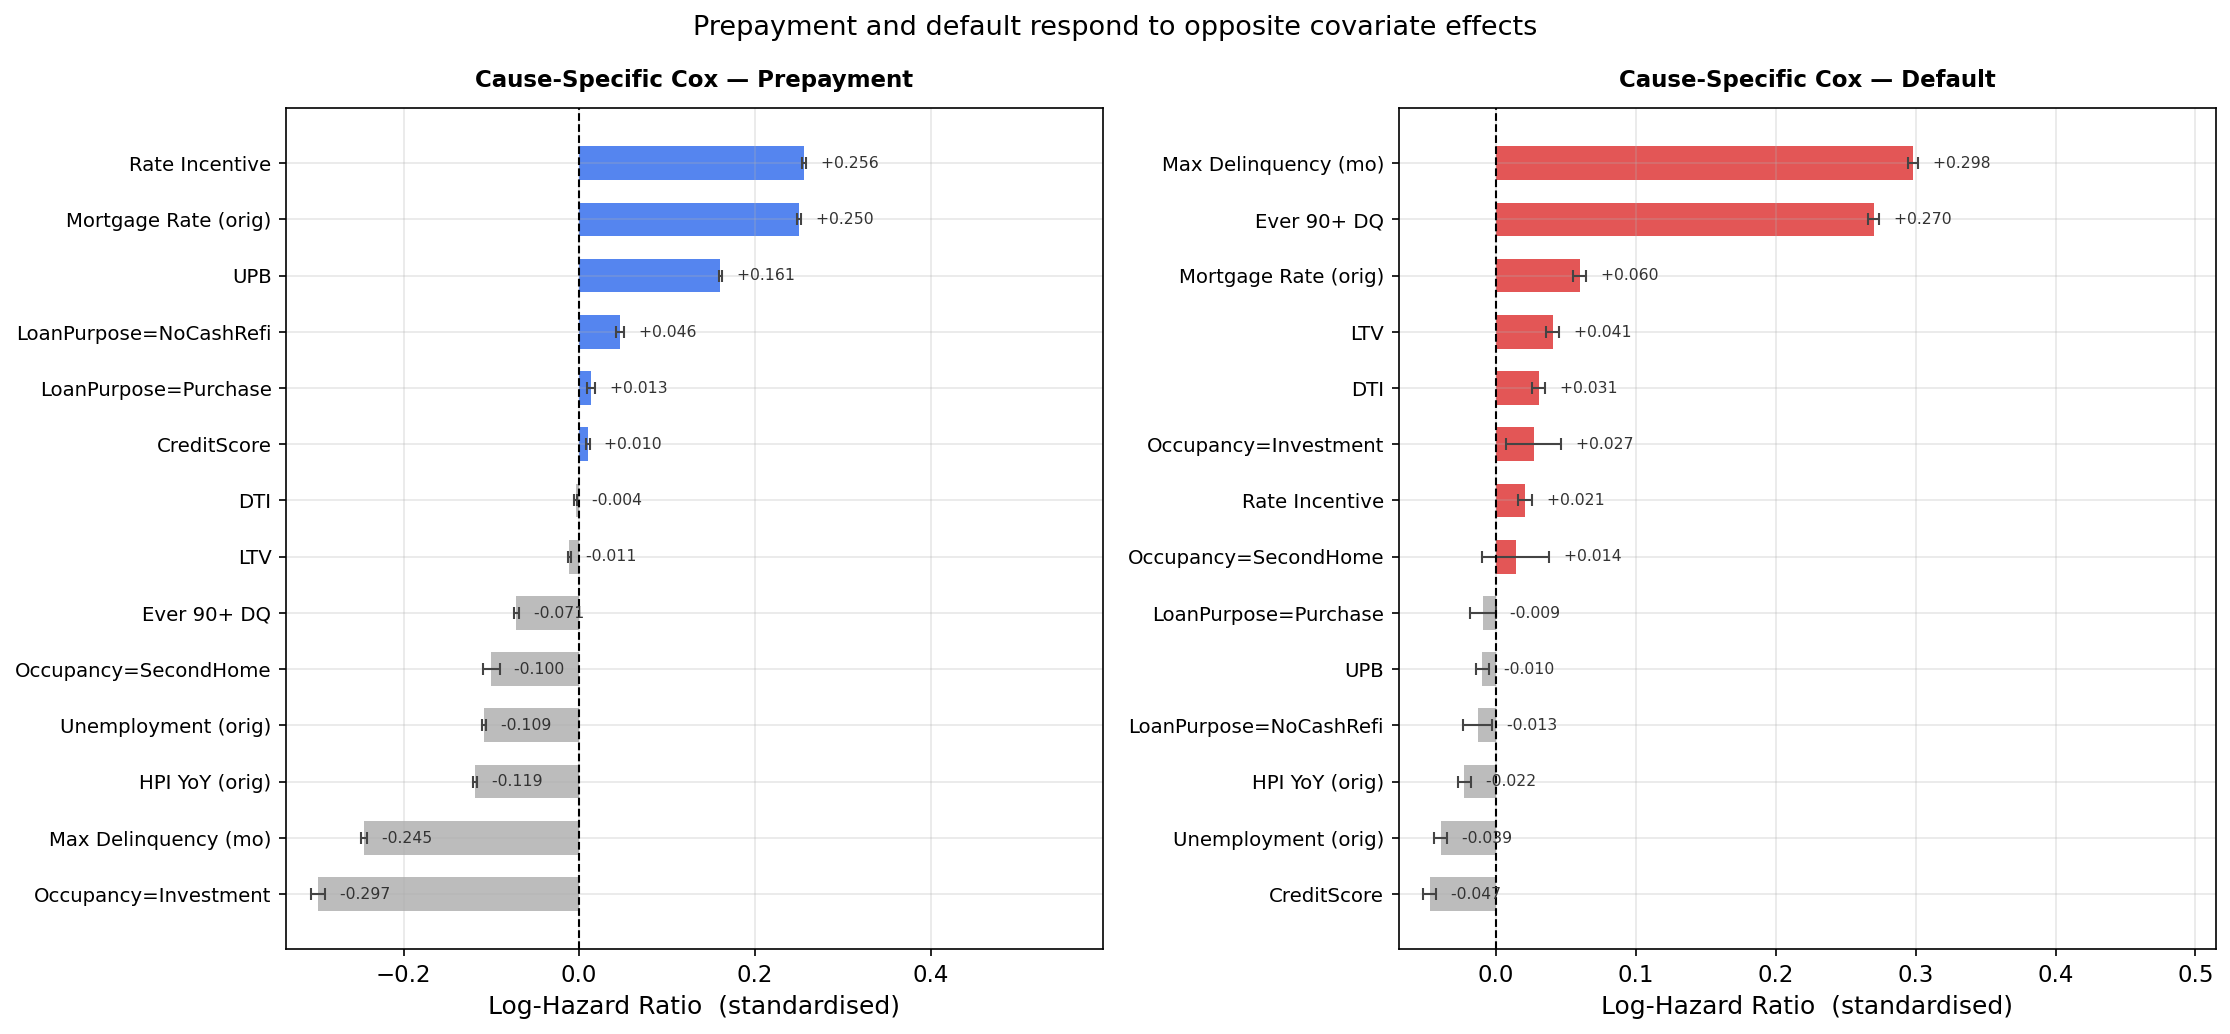
\includegraphics[width=\linewidth]{processed/E1_cause_specific_cox}
    \end{center}
\end{frame}

\begin{frame}{Four covariates flip sign across causes.}
    \vspace{0.2em}
    \begin{center}
    \small
    \textbf{Naive Cox vs.\ cause-specific coefficients}\\[4pt]
    \begin{tabular}{lrrrp{2.6cm}}
        \toprule
        \textbf{Covariate} & \textbf{Naive $\hat\beta$} & \textbf{Prepay $\hat\beta$} & \textbf{Default $\hat\beta$} & \\
        \midrule
        Rate incentive   & $+0.253$ & \textcolor{good}{$+0.256$} & $+0.021$                   & (pure prepay) \\
        UPB              & $+0.161$ & \textcolor{good}{$+0.161$} & $-0.010$                   & (pure prepay) \\
        \midrule
        FICO             & $+0.016$ & \textcolor{good}{$+0.010$} & \textcolor{bad}{$-0.047$}  & \textbf{opposite} \\
        LTV              & $-0.007$ & \textcolor{bad}{$-0.011$}  & \textcolor{good}{$+0.041$} & \textbf{opposite} \\
        Max Delinquency  & $-0.123$ & \textcolor{bad}{$-0.245$}  & \textcolor{good}{$+0.298$} & \textbf{opposite} \\
        Ever 90+ DQ      & $-0.035$ & \textcolor{bad}{$-0.071$}  & \textcolor{good}{$+0.270$} & \textbf{opposite} \\
        \bottomrule
    \end{tabular}
    \end{center}
    \vspace{0.3em}
    \begin{center}
        \small
        Each extra month delinquent raises default hazard by $35\%$ and cuts prepayment hazard by $22\%$
        --- yet the naive coefficient ($-0.123$) conceals both, collapsing a $+0.543$ spread to near zero.
    \end{center}
\end{frame}

\begin{frame}{Key Takeaways: E(i)}
    \begin{enumerate}\itemsep14pt
        \item Default and prepayment are competing risks --- a naive Cox model conflates both.
        \item \textbf{Kaplan--Meier overstates prepayment by up to $+$2.2\,pp; use Aalen--Johansen.}
        \item Vintage era dominates: 2007 cohort defaults at $6\times$ the long-run average.
        \item FICO drives default; rate incentive drives prepayment --- separate channels.
    \end{enumerate}
\end{frame}

% =========================================================================
\section{E(ii): Time-Varying Cox}
% =========================================================================

\begin{frame}
    \vfill
    \begin{center}
        {\color{accent}\rule{0.28\linewidth}{1.2pt}}\\[0.7em]
        {\Large\bfseries Part E(ii)}\\[0.5em]
        {\large Time-Varying Covariates in Mortgage Survival}\\[0.4em]
        {\small Andersen--Gill Cox Extension\enspace$\cdot$\enspace
                Live Rate Incentive\enspace$\cdot$\enspace Landmark C-index}\\[0.7em]
        {\color{accent}\rule{0.28\linewidth}{1.2pt}}
    \end{center}
    \vfill
\end{frame}

\begin{frame}{Static Cox vs.\ Andersen--Gill.}
    \begin{columns}[T,onlytextwidth]

        \column{0.50\textwidth}
        \begin{block}{Standard Cox (11 features)}
        \small\vspace{2pt}
        One row per loan; all covariates fixed at origination.
        Cannot track rate cycles, burnout, or equity build
        after origination.
        \vspace{2pt}
        \end{block}

        \vspace{0.5em}

        \begin{block}{Andersen--Gill (13 features)}
        \small\vspace{2pt}
        One row per loan-month; $\mathbf{x}_i(t)$ updated each period.
        Extends the same static base with the four time-varying
        features, tracking the full path of rate incentive and
        equity. 100K loans $\times$ ${\sim}47$ months $= 4.68$M intervals.
        \vspace{2pt}
        \end{block}

        \column{0.46\textwidth}
        \vspace{0.2em}
        \small\textbf{Time-varying features} --- updated every month
        \vspace{0.4em}

        \begin{tabular}{@{}p{2.5cm}p{4.1cm}@{}}
            \toprule
            \textbf{Feature} & \textbf{What it captures} \\
            \midrule
            \addlinespace[2pt]
            \texttt{rate\_incentive} & $r_{\text{orig}}{-}r_{\text{mkt}}(t)$: live option value to refinance; tracks rate cycles and burnout \\
            \addlinespace[4pt]
            \texttt{ELTV}            & equity from amortisation and HPI gains; high ELTV suppresses refi \\
            \addlinespace[4pt]
            \texttt{unemployment}    & macro labour cycle; proxies Fed easing in high-unemp periods \\
            \addlinespace[4pt]
            \texttt{hpi\_yoy}        & home-price appreciation unlocking cash-out refinancing \\
            \addlinespace[2pt]
            \bottomrule
        \end{tabular}

        \vspace{0.5em}
        \footnotesize $^*$\texttt{unemployment} and \texttt{hpi\_yoy} also in Standard Cox as origination-month snapshots.

    \end{columns}
\end{frame}

\begin{frame}{The Andersen--Gill model.}

    \textbf{Hazard function} \quad (identical in form to standard Cox)
    \[
        h_i(t) \;=\; h_0(t)\,\exp\!\bigl(\boldsymbol{\beta}^\top \mathbf{x}_i(t)\bigr)
    \]
    \small
    $\mathbf{x}_i(t)$ is the \textbf{current} covariate vector, updated each month.
    $\boldsymbol{\beta}$ is a single coefficient vector estimated across all loan-months.

    \medskip
    \normalsize\textbf{Log partial likelihood} \quad (maximised to obtain $\hat{\boldsymbol{\beta}}$)
    \[
        \ell(\boldsymbol{\beta}) \;=\;
        \sum_{i:\,\delta_i=1}
        \Biggl[
            \underbrace{\boldsymbol{\beta}^\top \mathbf{x}_i(t_i)}_{\substack{\text{log-score of}\\\text{the prepaying loan}}}
            \;-\;\log
            \underbrace{\sum_{j \in \mathcal{R}(t_i)}
            \exp\!\bigl(\boldsymbol{\beta}^\top \mathbf{x}_j(t_i)\bigr)}_{\substack{\text{sum over all loan-months}\\\text{active at }t_i}}
        \Biggr]
    \]
    \small
    At each event: \textit{given a prepayment at $t_i$, what is the probability it was loan $i$
    rather than any other active loan?}
    Maximising $\ell$ estimates $\hat{\boldsymbol{\beta}}$ without specifying $h_0(t)$.

\end{frame}

\begin{frame}{Time-varying feature trajectories by vintage.}
    \begin{center}
        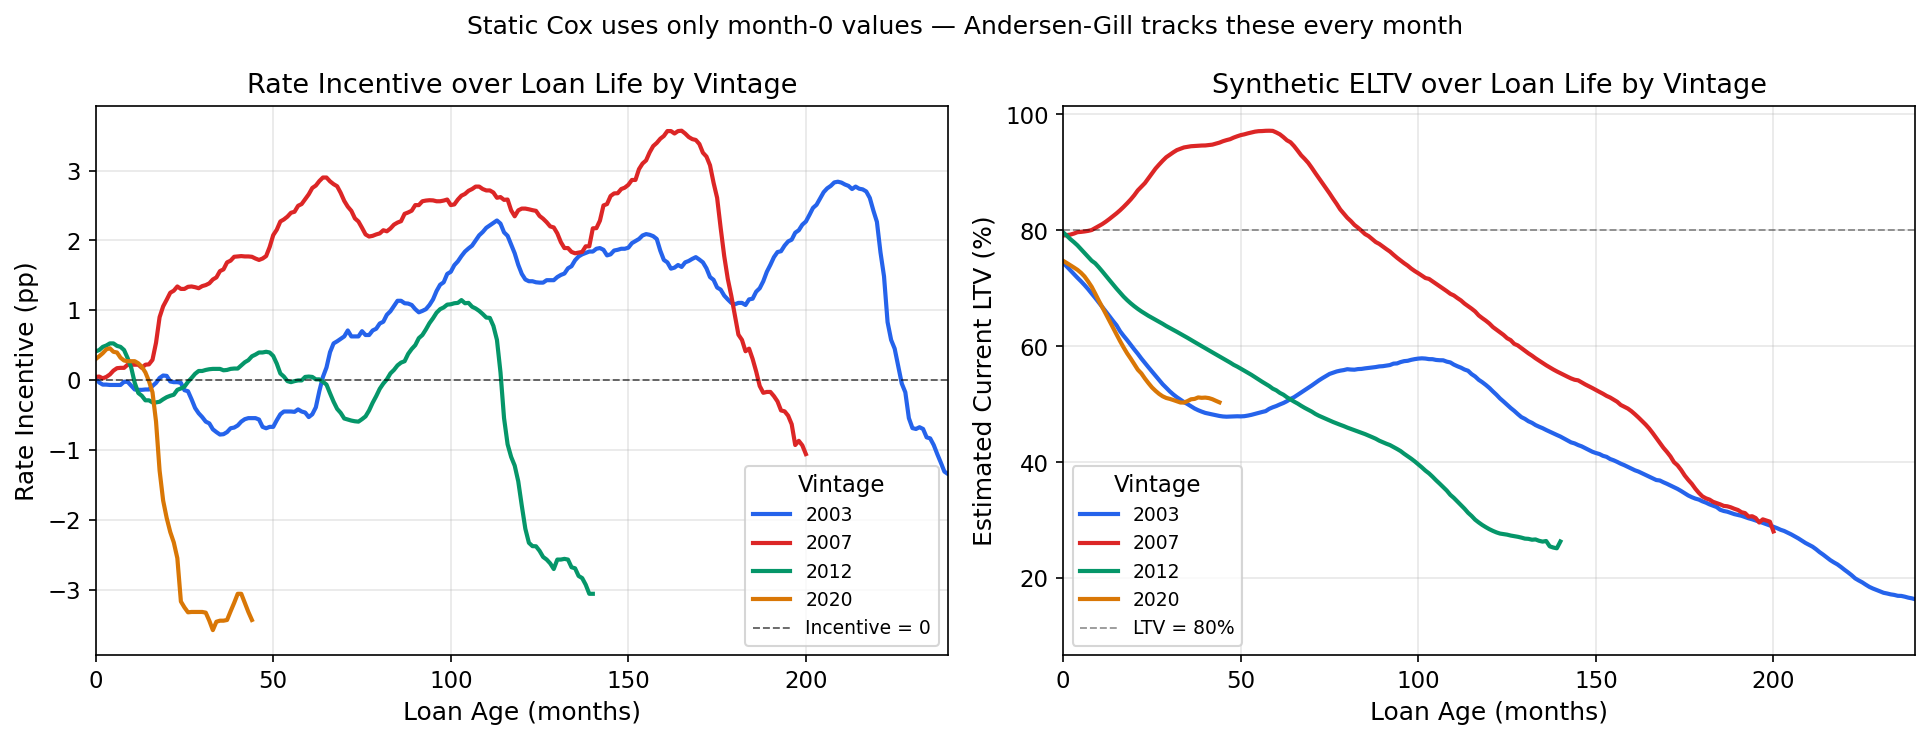
\includegraphics[width=0.90\linewidth]{processed/Eii_tv_feature_trajectories}
    \end{center}
    \vspace{-0.5em}
    \begin{center}
        \small
        Static Cox uses only month-0 values --- Andersen-Gill tracks these every month.
    \end{center}
\end{frame}

\begin{frame}{Static vs.\ TV Cox coefficient comparison.}
    \begin{center}
        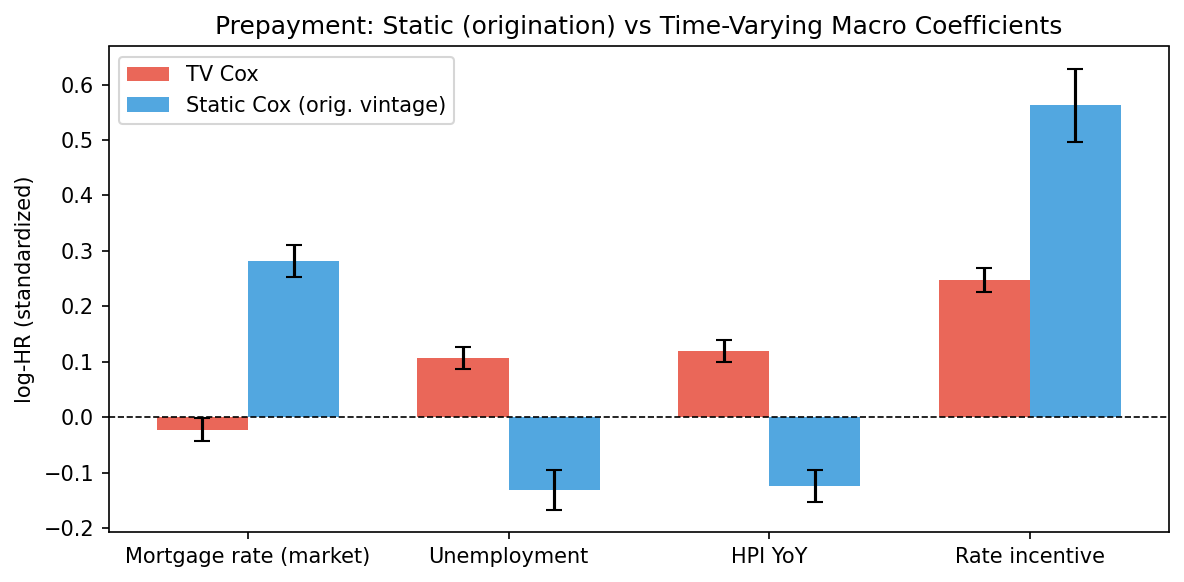
\includegraphics[width=0.92\linewidth]{processed/Eii_static_vs_tv}
    \end{center}
    \vspace{-0.3em}
    \small
    \begin{itemize}\itemsep2pt
        \item \texttt{rate\_incentive}: dominant positive predictor in TV Cox; near zero at origination, absent from Static Cox
        \item Macro signals (unemployment, HPI) flip sign --- vintage-era snapshots capture a different regime than monthly values
    \end{itemize}
\end{frame}

\begin{frame}{Landmark C-index: TV Cox leads to $T{=}60$, then reverses.}
    \begin{columns}[c,onlytextwidth]
        \column{0.56\textwidth}
        \begin{center}
            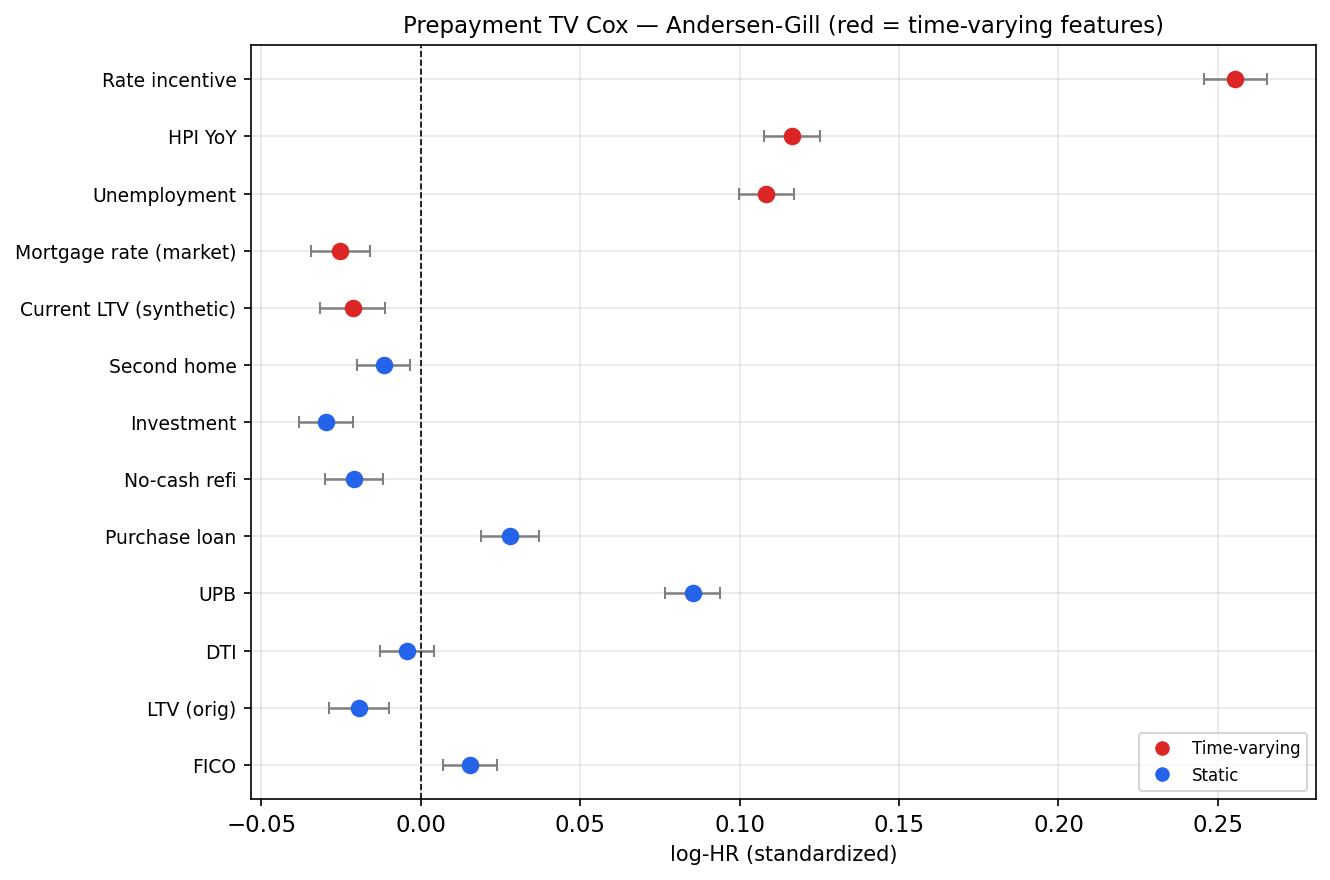
\includegraphics[width=\linewidth]{processed/Eii_tv_cox_forest}
        \end{center}

        \column{0.42\textwidth}
        \begin{center}
        \small
        \textbf{Landmark C-index}\\[2pt]
        $C(t^*) = P\!\bigl(\hat{h}_i(t^*)>\hat{h}_j(t^*)\mid T_i\le t^*<T_j\bigr)$\\[10pt]
        \begin{tabular}{lccc}
            \toprule
            Horizon & Static & \textbf{TV} & $\Delta$ \\
            \midrule
            $T=12$ & 0.609 & \textbf{0.681} & $+0.072$ \\
            $T=24$ & 0.627 & \textbf{0.687} & $+0.060$ \\
            $T=36$ & 0.630 & \textbf{0.675} & $+0.045$ \\
            $T=60$ & 0.625 & \textbf{0.646} & $+0.021$ \\
            $T=84$ & \textbf{0.623} & 0.605 & \textcolor{bad}{$-0.018$} \\
            $T=120$ & \textbf{0.620} & 0.583 & \textcolor{bad}{$-0.037$} \\
            \bottomrule
        \end{tabular}
        \end{center}
    \end{columns}
\end{frame}

\begin{frame}{Key Takeaways: E(ii)}
    \begin{enumerate}\itemsep14pt
        \item Monthly-updated covariates add real information ($+$1,996 log-likelihood gain).
        \item \textbf{TV Cox leads at short/medium horizons: $+0.072$ at $T{=}12$, $+0.021$ at $T{=}60$.}
        \item \textbf{TV Cox degrades beyond $T{\approx}70$ months --- use a landmark super-model.}
        \item Rate incentive is the key driver; macro coefficients require careful inspection.
    \end{enumerate}
\end{frame}

% =========================================================================
\section{E(iii): Neural Survival Models}
% =========================================================================

\begin{frame}
    \vfill
    \begin{center}
        {\color{accent}\rule{0.28\linewidth}{1.2pt}}\\[0.7em]
        {\Large\bfseries Part E(iii)}\\[0.5em]
        {\large Neural Survival Models: LongitudinalDeepHit}\\[0.4em]
        {\small Transformer Encoder\enspace$\cdot$\enspace
                Competing-Risk CIFs\enspace$\cdot$\enspace
                Gradient Sensitivity}\\[0.7em]
        {\color{accent}\rule{0.28\linewidth}{1.2pt}}
    \end{center}
    \vfill
\end{frame}

\begin{frame}{Why go beyond Cox?}
    \begin{columns}[T,onlytextwidth]
        \column{0.48\textwidth}
        \begin{block}{Cox / Andersen-Gill limitations}
        \small
        \begin{itemize}\itemsep4pt
            \item Proportional hazards: covariate effect is \textbf{constant over time}
            \item Single scalar score --- cannot model the \textbf{S-curve shape} of prepayment
            \item Competing risks require separate model fits; no shared representation
            \item Cannot exploit the \textbf{sequence structure} of monthly covariate history
        \end{itemize}
        \end{block}

        \column{0.48\textwidth}
        \begin{block}{What a sequence model can do}
        \small
        \begin{itemize}\itemsep4pt
            \item Read the full monthly path $[\mathbf{x}_1, \dots, \mathbf{x}_T]$ --- \textbf{burnout is encoded}
            \item Produce nonlinear, time-varying hazard rates $\lambda_k(t \mid \mathbf{x})$
            \item Model prepayment and default \textbf{jointly} via shared encoder
            \item Attention weights identify \textbf{which months} drive the prediction
        \end{itemize}
        \end{block}
    \end{columns}
\end{frame}

\begin{frame}{Architecture rationale.}
    \begin{columns}[T,onlytextwidth]
        \column{0.46\textwidth}
        \begin{alertblock}{Alternatives rejected}
        \small
        \begin{itemize}\itemsep4pt
            \item \textbf{LSTM} --- vanishing gradients at $T{=}120$; attends only to adjacent months; hard to interpret
            \item \textbf{Single-context head} --- no time index in head; near-constant hazard curve; gradient flows only through last hidden state
            \item \textbf{Two separate models} --- violates independent censoring (defaulted loans are riskiest borrowers, not random exits); loses shared macro signal
        \end{itemize}
        \end{alertblock}

        \column{0.50\textwidth}
        \begin{block}{Why this combination}
        \small
        \begin{itemize}\itemsep4pt
            \item \textbf{Causal Transformer} --- reaches any past month in one attention step; gradient flows through every position; weights are interpretable
            \item \textbf{Per-timestep head} --- $\lambda(t){=}\text{head}(h_t)$: hazard conditioned on full causal history $\mathbf{x}_1\!\dots\mathbf{x}_t$; every month trained independently
            \item \textbf{Joint encoder} --- shared representation captures that the same macro shock raises default and suppresses prepayment; chain product enforces $\text{CIF}_1{+}\text{CIF}_2{+}S{=}1$
        \end{itemize}
        \end{block}
    \end{columns}
\end{frame}

\begin{frame}{LongitudinalDeepHit architecture.}
    \begin{columns}[T,onlytextwidth]
        \column{0.52\textwidth}
        \begin{block}{Architecture}
        \small
        \begin{tabular}{@{}ll@{}}
            \textbf{Input}  & $(B,\, T_{\max}{=}120,\, D{=}13)$ padded sequences \\
            \textbf{Proj.}  & Linear $D \to d_{\text{model}}{=}64$ \\
            \textbf{PE}     & Sinusoidal positional encoding on loan age \\
            \textbf{Enc.}   & $\times 2$ pre-norm layers, 4 heads, causal mask \\
            \textbf{Head 1} & FC $64\!\to\!64\!\to\!1$ per $h_t$, Sigmoid $\Rightarrow \lambda_1(t)$ \\
            \textbf{Head 2} & FC $64\!\to\!64\!\to\!1$ per $h_t$, Sigmoid $\Rightarrow \lambda_2(t)$ \\
            \textbf{CIFs}   & Competing-risk chain product \\
        \end{tabular}
        \end{block}

        \vspace{0.1em}
        \begin{block}{Competing-risk CIFs}
        \footnotesize
        \vspace{-0.9em}
        \begin{align*}
            \text{CIF}_k(t) &= \textstyle\sum_{s=1}^{t} \lambda_k(s)\cdot S(s-1) \\[-3pt]
            S(t) &= \textstyle\prod_{s=1}^{t}(1-\lambda_1(s))(1-\lambda_2(s))
        \end{align*}
        \vspace{-0.9em}
        Guarantees $\text{CIF}_1 + \text{CIF}_2 + S = 1$ at every $t$.
        \end{block}

        \column{0.44\textwidth}
        \begin{block}{Training objective}
        \footnotesize
        \vspace{-0.3em}
        \[
            \mathcal{L} = \mathcal{L}_{\text{NLL}} + \alpha\,\mathcal{L}_{\text{rank}},
            \quad \alpha=0.2
        \]
        \vspace{-0.4em}
        \textbf{NLL}: discrete-time cause-specific likelihood\\[1pt]
        \textbf{Ranking}: soft pairwise concordance (DeepHit-style)\\[3pt]
        \begin{tabular}{@{}ll@{}}
            Params & 76,290 \\
            Data   & 101K loans, 4.5M rows \\
            Epochs & 41 \;(best ep.\,29) \\
            LR     & $3\!\times\!10^{-4}$, cosine \\
            Loss   & $11.30 \to 11.28$ \\
            Rank   & $1.97 \to 1.84$ \\
        \end{tabular}
        \end{block}

        \vspace{0.1em}
        \begin{block}{Data treatment}
        \footnotesize
        Each loan $\to$ 13-feature monthly sequence,\\
        zero-padded to $T_{\max}{=}120$ after exit.\\[2pt]
        Labels: prepayment\,=\,1, default\,=\,2, censored\,=\,0.\\[2pt]
        Causal mask; 80/20 train--test split.
        \end{block}
    \end{columns}
\end{frame}

\begin{frame}{Training dynamics: Negative Log Likelihood collapse and ranking loss.}
    \begin{center}
        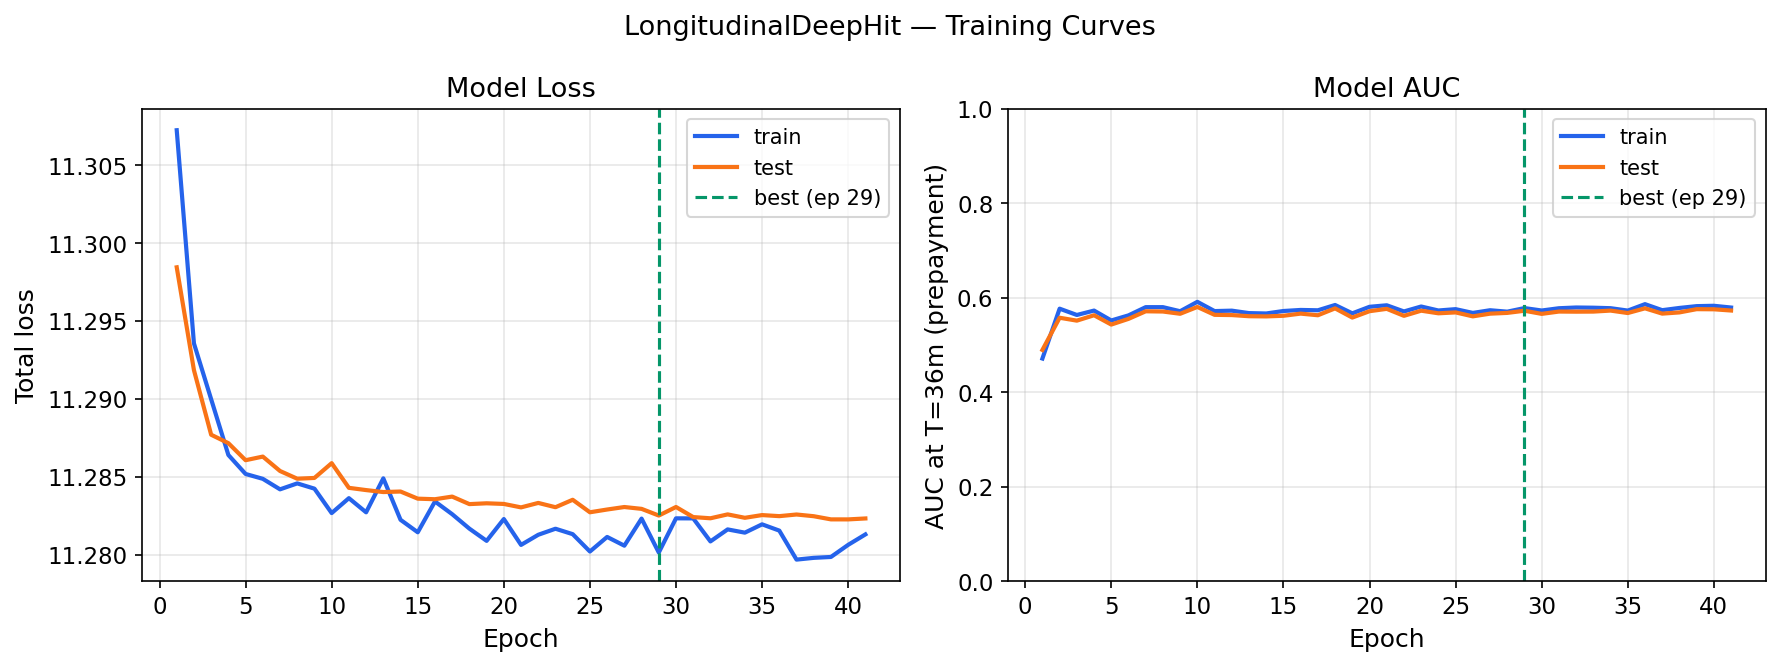
\includegraphics[width=0.88\linewidth]{processed/Eiii_training_curves}
    \end{center}
    \vspace{-0.1em}
    \begin{itemize}\itemsep2pt\footnotesize
        \item \textbf{NLL freezes}: 1.6\% event rate means predicting near-zero hazard for everyone already minimises the loss --- rare-event gradients too weak to improve further.
        \item \textbf{Cox immune}: partial likelihood only ranks loans at event times, never predicts absolute hazard --- no trivial solution under class imbalance.
        \item \textbf{AUC preserved}: ranking loss descends steadily, ordering loans by relative risk despite collapsed hazard values.
    \end{itemize}
\end{frame}

\begin{frame}{Gradient sensitivity by cause.}
    \begin{center}
        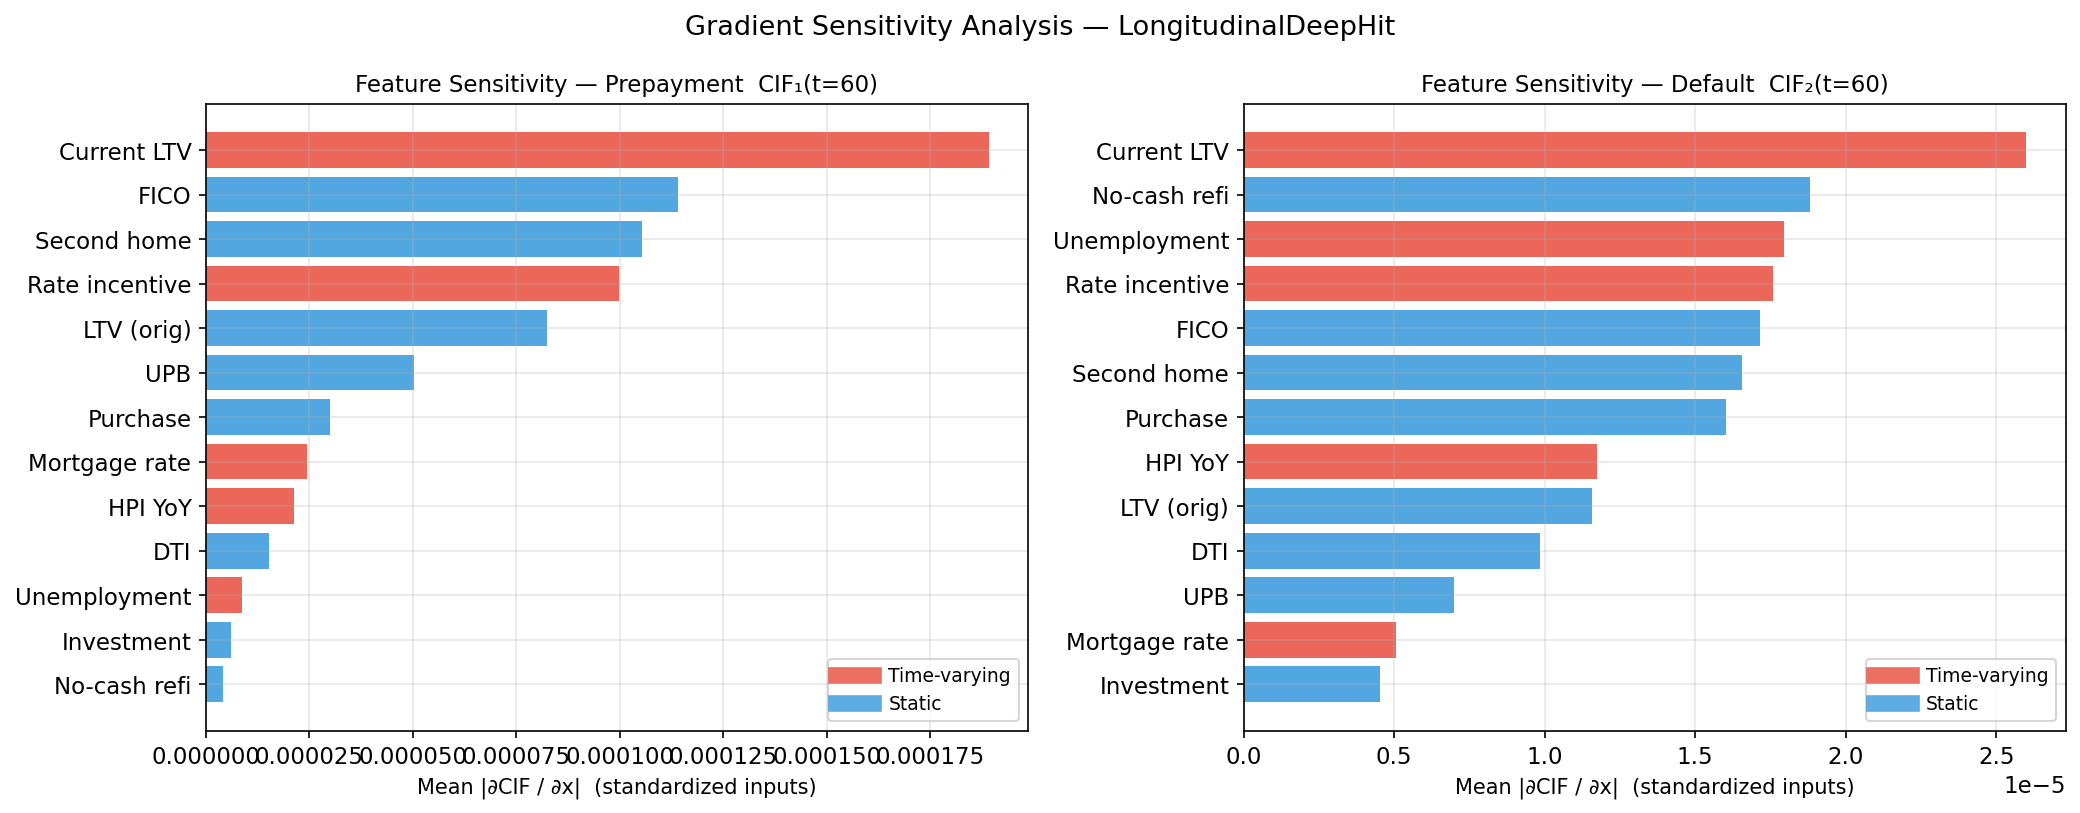
\includegraphics[width=0.84\linewidth]{processed/Eiii_gradient_sensitivity}
    \end{center}
    \vspace{-0.4em}
    \begin{center}
        \small
        \textcolor{bad}{Red} = time-varying features. \quad \textcolor{accent}{Blue} = static features.\\
        Dynamic features rank above static for prepayment; 
        
        FICO and unemployment lead for default; consistent with cause-specific Cox in E(i).
    \end{center}
\end{frame}

\begin{frame}{Feature importance over the loan lifecycle.}
    \begin{center}
        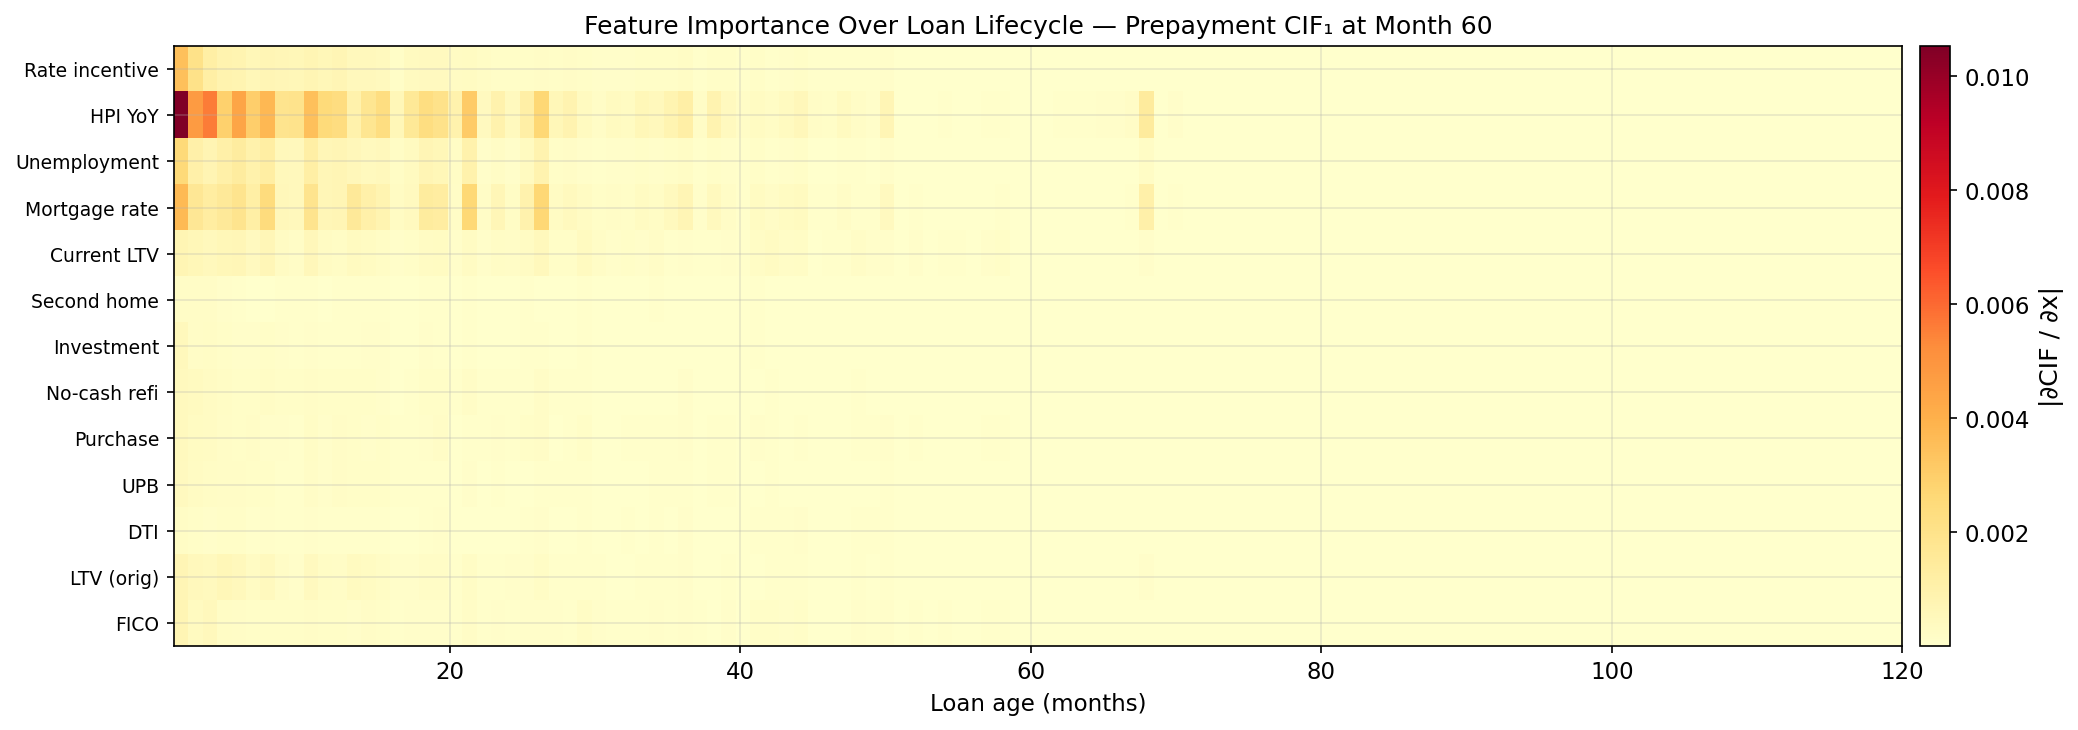
\includegraphics[width=0.92\linewidth]{processed/Eiii_sensitivity_over_time}
    \end{center}
    \vspace{-0.4em}
    \begin{center}
        \small
        \texttt{rate\_incentive} and \texttt{Mortgage rate} dominates, especially in early months; 
  
    \end{center}
\end{frame}

\begin{frame}{Model performance vs.\ DeepCox.}
    \begin{center}
        \small\textbf{Prepayment CIF$_1$ --- AUC at fixed horizons}\\[4pt]
        \begin{tabular}{lcccc}
            \toprule
            \textbf{Model} & \textbf{T=12} & \textbf{T=24} & \textbf{T=36} & \textbf{T=60} \\
            \midrule
            Part D DeepCox$^\dagger$ & \textcolor{good}{\textbf{0.684}} & \textcolor{good}{\textbf{0.701}} & \textcolor{good}{\textbf{0.721}} & \textcolor{good}{\textbf{0.729}} \\
            DeepHit (20K)$^\ddagger$ & 0.641 & 0.622 & 0.572 & 0.515 \\
            \bottomrule
        \end{tabular}

        \vspace{8pt}
        \small\textbf{Default CIF$_2$ --- AUC at fixed horizons}\\[4pt]
        \begin{tabular}{lcccc}
            \toprule
            \textbf{Model} & \textbf{T=12} & \textbf{T=24} & \textbf{T=36} & \textbf{T=60} \\
            \midrule
            Part D DeepCox$^\dagger$  & 0.684 & 0.701 & \textcolor{good}{\textbf{0.721}} & \textcolor{good}{\textbf{0.729}} \\
            DeepHit (20K)$^\ddagger$  & \textcolor{good}{\textbf{0.687}} & \textcolor{good}{\textbf{0.708}} & 0.707 & 0.726 \\
            \bottomrule
        \end{tabular}
        \vspace{3pt}\\
        \tiny $^\dagger$\,597K canonical \quad $^\ddagger$\,20K hold-out \quad \textcolor{good}{\textbf{green}} = better
    \end{center}

    \vfill
    \begin{center}
        \small
        Prepayment: DeepCox leads at all horizons (NLL collapse hurts long-horizon calibration).\\
        Default: DeepHit leads at T=12 and T=24 with \textbf{6$\times$ fewer} training loans.
    \end{center}
\end{frame}

\begin{frame}{Key Takeaways: E(iii)}
    \begin{enumerate}\itemsep14pt
        \item Default AUC matches DeepCox with $6\times$ fewer training loans.
        \item Gradient sensitivity replicates Cox findings: rate incentive drives prepayment, FICO drives default.
        \item Feature importance shifts over the loan lifecycle --- unique to sequence models.
        \item \textbf{Limitation: defaults are rare (1.6\%), so the model learns to predict near-zero hazard for everyone --- AUC is preserved but absolute probabilities are unreliable; fix via focal-loss upweighting.}
    \end{enumerate}
\end{frame}

% =========================================================================
\section{E(iv): Scenario Analysis}
% =========================================================================

\begin{frame}
    \vfill
    \begin{center}
        {\color{accent}\rule{0.28\linewidth}{1.2pt}}\\[0.7em]
        {\Large\bfseries Part E(iv)}\\[0.5em]
        {\large Scenario Analysis: MBS Prepayment under Rate Shocks}\\[0.4em]
        {\small TV Cox Rate Channel\enspace$\cdot$\enspace
                Survival Curves\enspace$\cdot$\enspace
                Monte Carlo MBS Pricing}\\[0.7em]
        {\color{accent}\rule{0.28\linewidth}{1.2pt}}
    \end{center}
    \vfill
\end{frame}

\begin{frame}{TV Cox: direct rate channel for scenario analysis.}
    \begin{block}{Why TV Cox (E(ii)) is the primary model}
    \small
    \texttt{rate\_incentive} $= r_{\text{orig}} - r_{\text{market}}(t)$ is a
    \textbf{direct time-varying covariate}.\\[6pt]
    A $\Delta r$\,bp market rate shock immediately shifts the incentive by $-\Delta r/100$\,pp,
    giving an analytic hazard response:
    \[
        \Delta\log h(t) = \hat\beta_{\text{ri}} \times \frac{-\Delta r}{100},
        \qquad \hat\beta_{\text{ri}} = 0.041 \text{ (HR} = 1.042 \text{ per 100\,bp)}
    \]
    The calibrated baseline hazard $\hat{H}_0(t)$ produces realistic $S(t)$, CPR, WAL,
    and price --- no approximation needed.\\[6pt]

    \end{block}
    \vspace{0.8em}
    \begin{center}
        \small
        Representative loan: \$300K, 5.0\% coupon, baseline market rate 5.3\% (median, 1999--2025).\\
        Scenarios: $\pm$100, $\pm$200, $\pm$300\,bp --- covering the BCBS standard stress range.
    \end{center}
\end{frame}

\begin{frame}{Shock sensitivity: TV Cox matches the analytic formula.}
    \begin{center}
        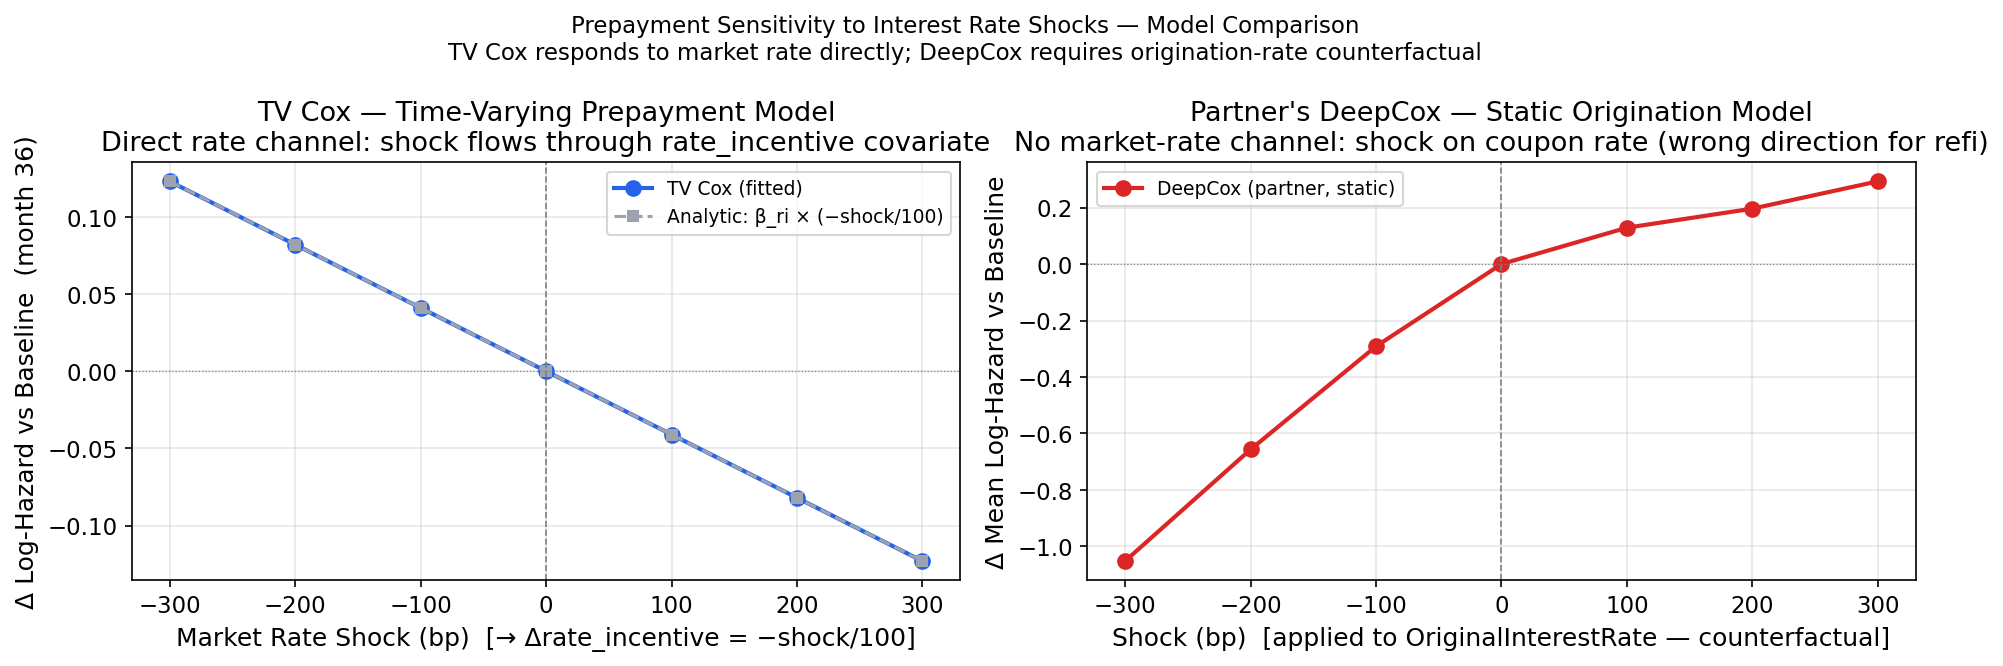
\includegraphics[width=0.64\linewidth]{processed/Eiv_shock_comparison}
    \end{center}
    \vspace{-0.4em}
    \begin{center}
        \small
        Each 100\,bp rate cut increases the prepayment hazard by 4.2\%; a 300\,bp cut raises it by $+0.123$ in log terms.\\
        The model response matches the closed-form prediction exactly --- no simulation needed, fully auditable.
    \end{center}
\end{frame}

\begin{frame}{Survival curves under seven rate scenarios.}
    \begin{columns}[c,onlytextwidth]
        \column{0.62\textwidth}
        \begin{center}
            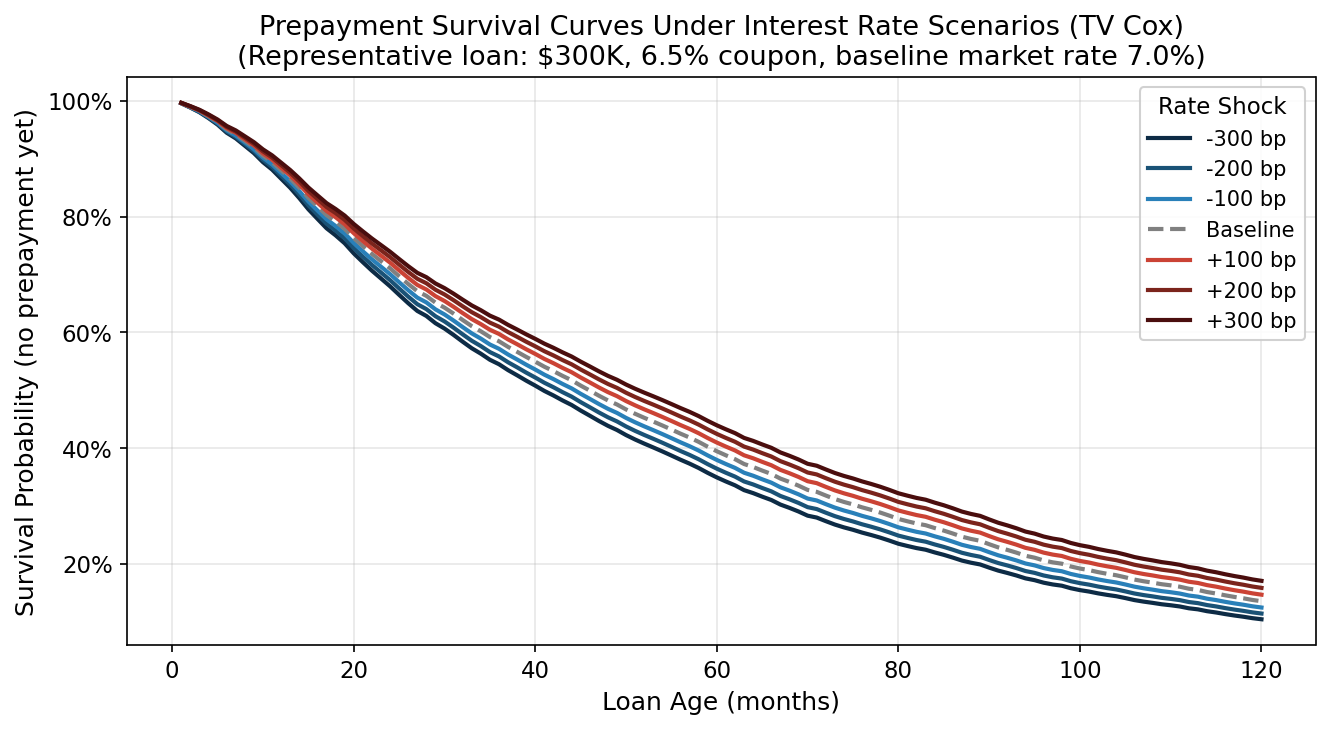
\includegraphics[width=\linewidth]{processed/Eiv_survival_curves}
        \end{center}

        \column{0.34\textwidth}
        \small
        \begin{tabular}{@{}lcc@{}}
            \toprule
            Scenario & \makecell{10-yr\\Survival} & \makecell{Median\\Prepay (mo.)} \\
            \midrule
            $-300$\,bp & 10.2\% & 41 \\
            $-200$\,bp & 11.2\% & 43 \\
            $-100$\,bp & 12.2\% & 45 \\
            Baseline   & 13.3\% & 46 \\
            $+100$\,bp & 14.4\% & 48 \\
            $+200$\,bp & 15.6\% & 50 \\
            $+300$\,bp & 16.8\% & 51 \\
            \bottomrule
        \end{tabular}
    \end{columns}
\end{frame}


\begin{frame}{MBS: Weighted Average Life, MBS price, and negative convexity.}
    \begin{columns}[c,onlytextwidth]
        \column{0.60\textwidth}
        \begin{center}
            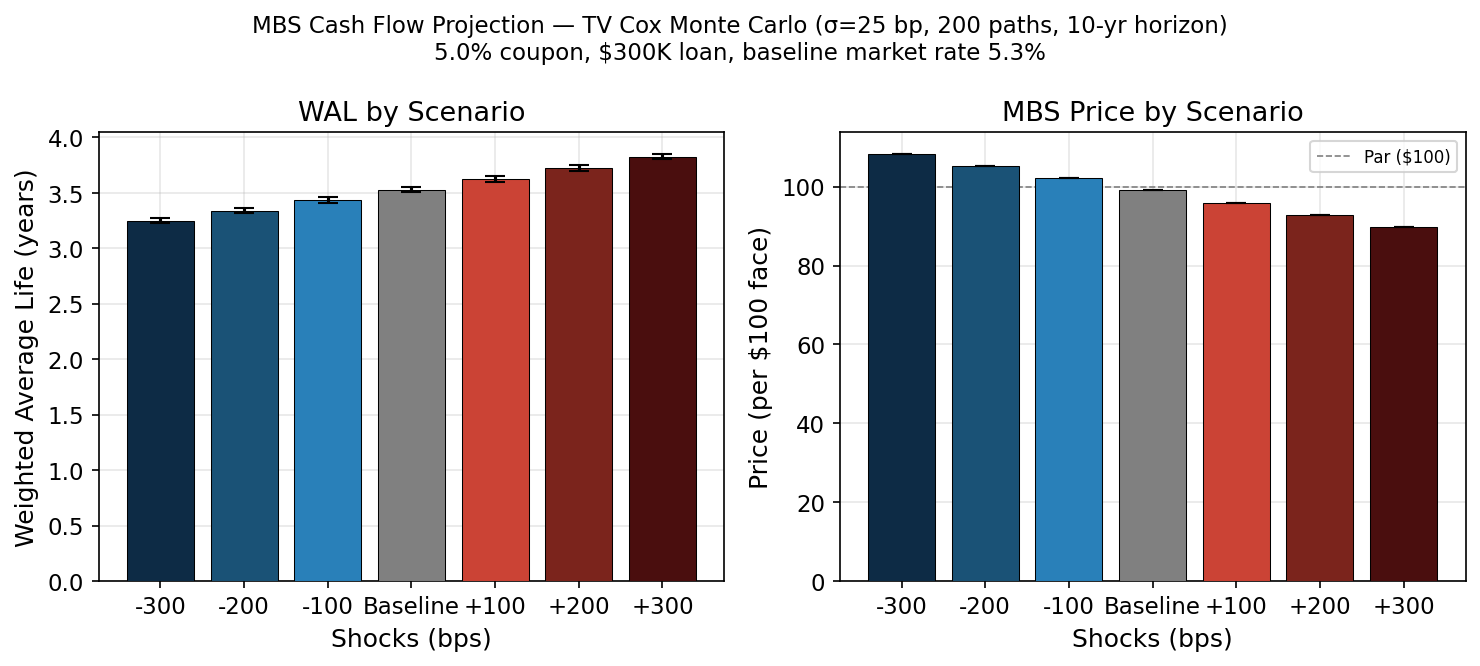
\includegraphics[width=\linewidth]{processed/Eiv_mbs_cashflows}
        \end{center}

        \column{0.36\textwidth}
        \small
        \begin{tabular}{@{}lrr@{}}
            \toprule
            Scenario & WAL\,(yr) & Price\,(\$) \\
            \midrule
            $-300$\,bp & 3.25 & 108.32 \\
            $-200$\,bp & 3.34 & 105.26 \\
            $-100$\,bp & 3.43 & 102.17 \\
            Baseline   & 3.53 & \phantom{0}99.07 \\
            $+100$\,bp & 3.63 & \phantom{0}95.96 \\
            $+200$\,bp & 3.73 & \phantom{0}92.86 \\
            $+300$\,bp & 3.83 & \phantom{0}89.77 \\
            \bottomrule
        \end{tabular}
        \vspace{0.4em}

        \textbf{Negative convexity}: when rates fall, borrowers prepay and return principal \emph{at par}, capping price upside. Price gain ($-300$\,bp: \$9.25) $<$ loss ($+300$\,bp: \$9.30).\\[4pt]
        MC: 200 paths, $\sigma{=}25$\,bp.
    \end{columns}
\end{frame}

\begin{frame}{Key Takeaways: E(iv)}
    \begin{enumerate}\itemsep12pt
        \item \textbf{TV Cox has a linear rate channel}: every 100\,bp rate cut adds the same $+4.2\%$ to prepayment hazard --- equal steps in rate produce equal steps in response, making results predictable and fully explainable.
        \item \textbf{Negative convexity confirmed}: when rates fall, borrowers prepay at par, capping price upside (\$9.25 gain $<$ \$9.30 loss at $\pm$300\,bp).
    \end{enumerate}
\end{frame}

% ---- Final thank you -------------------------------------------------------
\begin{frame}[plain]
    \vspace*{2em}
    \begin{center}
        {\Huge \textbf{Thank you}}\\[1.5em]
        {\Large Questions?}\\[2.5em]
        \small
        Andersen \& Gill (1982) \textit{Ann.\ Stat.}\enspace$\cdot$\enspace
        Fine \& Gray (1999) \textit{JASA}\enspace$\cdot$\enspace
        Lee et al.\ (2018) \textit{DeepHit}\enspace$\cdot$\enspace
        Sadhwani et al.\ (2021) \textit{J.\ Fin.\ Econometrics}\enspace$\cdot$\enspace
        BCBS (2019)
    \end{center}
\end{frame}

\end{document}
